\chapter{บทนำ}

\par{
ก่อนจะถึงในรายละเอียดข้างต้น 
ในส่วนแรกจะกล่าวถึงประวัติและความเป็นมาของ
ระบบการคำนวณอันเป็นที่มาของสถาปัตยกรรมคอมพิวเตอร์
}

\par{
Charles Babbage เป็นศาสตราจารย์ในสาขาคณิตศาสตร์ที่มหาวิทยาลัย 
Cambridge ในช่วง 1827 ถึง 1839 ซึ่งถูกยกย่องว่า
เป็นบิดาแห่งคอมพิวเตอร์ (father of the computer) 
\cite{halacy1970charles}
เนื่องจากเป็นผู้คิดค้นเครื่องคำนวณแบบจักรกลเป็นผลสำเร็จเป็นคนแรก อัน
นำมาซึ่งในการออกแบบเครื่องคำนวณในรูปแบบต่าง ๆ ที่มีความซับซ้อนมากยิ่งขึ้น 
หนึ่งในเครื่องจักรการคำนวณที่จะกล่าวถึงคือ Different Engine 
(ถูกออกแบบในปี 1823) ดังแสดงในรูปที่ 
\ref{fig_babbage_difference_engine}
}
%
%
\begin{figure}[h]
\centering
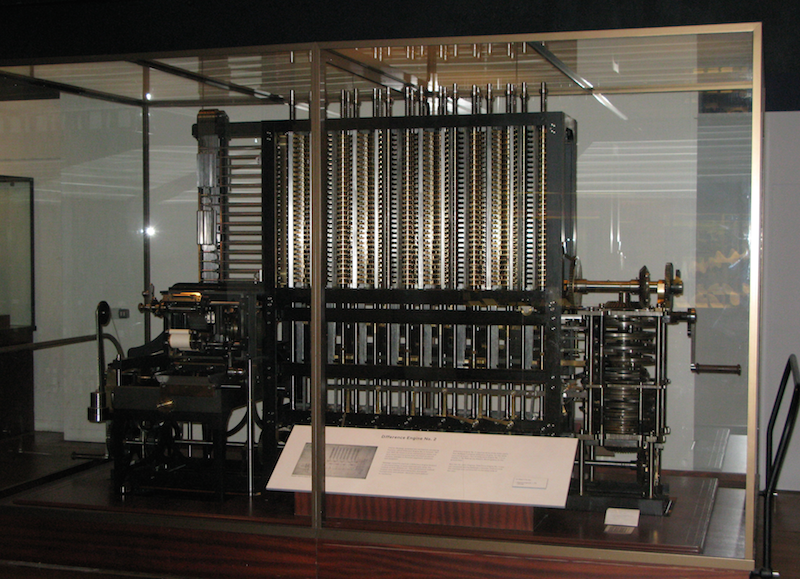
\includegraphics[width=0.75\textwidth]{fig/Babbage_Difference_Engine.png}
\caption{Different Engine ที่ถูกจัดแสดงใน London Science Museum}
\label{fig_babbage_difference_engine}
\end{figure}
%
%
\par{
จุดมุ่งหมายของการออกแบบ Different Engine 
คือต้องการใช้เครื่องจักรในการแก้ปัญหาทางคณิตศาสตร์ที่มีหลัก
ในการแก้เป็นแบบการวนซ้ำ (Iteration) ซึ่งปัญหาคณิตศาสตร์
ดังกล่าวคือ การหาค่าของสมการพหุนามด้วย 
Finite Difference Method ตัวอย่างเช่น  
กำหนดให้  $f(x) เป็นฟังก์ชั่นพหุนาม โดยที่มีค่าเป็น 
$x^2 + x + 33$ ดังนั้น
%
\begin{align}
f(x)&=x^2+x+33\\
d_1(x)&=f(x) - f(x-1) = 2x\\
d_2(x)&=d_1(x) - d_1(x-1) = 2
\end{align}
%
ในทางย้อนกลับจากข้างต้นจะได้ว่า
%
\begin{align}
d_2(x)&=2\\
d_1(x)&=d_1(x-1) + d_2(x) \\
f(x)&=f(x-1) + d_1(x)
\end{align}
%
จากชุดของสมการข้างต้นสามารถสร้างตาราง
ในการคำนวณค่าของพหุนามสำหรับค่าที่กำหนดให้ 
$x$ ใด ๆ ดังแสดงในตารางที่ 
\ref{tab:finite_difference_method}
%
\begin{table}
\caption{ตัวอย่างปัญหาที่แก้ด้วยวิธี Finite Difference Method}
\label{tab:finite_difference_method}
\begin{center}
\begin{tabular}{|l|c|c|c|c|c|c|c|}
$x$ & 0 & 1 & 2 & 3 & 4 & 5 & 6 \\
\hline
$d_2(x) & & & 2 & 2 & 2 & 2 & 2 \\
$d_1(x) & & 2 & 4 & 6 & 8 & 10 & 12 \\
$f(x) & 33 & 35 & 39 & 45 & 53 & 63 & 75 
\hline
\end{tabular}
\end{center}
\end{table}
%
กรณีที่ต้องการหาค่าของ $f(x)$ 
เมื่อ $x$ มีค่าเป็น 3 สามารถคำนวณได้จาก 
ค่าของ $f(2)$ และ $d_1(2)$ ดังนี้ 
%
\begin{align}
d_2(3)&=2\\
d_1(3)&=d_1(2) + d_2(3) \\
&= 4 + 2 = 6 \\
f(3)&=f(2) + d_1(3) \\
&= 39 + 6 = 45
\end{align}
%
จะเห็นได้ว่าการคำนวณหาของพหุนามนั้นเป็นการ
ท ำบวกซ้ำ ๆ กันของค่าที่คำนวณก่อนหน้า 
ซึ่งเป็นพื้นฐานในการแก้ปัญหาด้วยวิธีการวนซ้ำ 
การออกแบบเครื่องจักรกล Different Engine ของ 
Babbage สามารถสร้างขึ้นและทำงานได้จริงในปี 1855 
โดย Scheutz โดยเครื่องจักรดังกล่าว 
สามารถคำนวณพหุนามได้ถึงดีกรีที่ 6 
}

